\let\negmedspace\undefined
\let\negthickspace\undefined
\documentclass[journal,12pt,twocolumn]{IEEEtran}
\usepackage{gensymb}
\usepackage{amssymb}
\usepackage[cmex10]{amsmath}
\usepackage{amsthm}
\usepackage[export]{adjustbox}
\usepackage{bm}
\usepackage{longtable}
\usepackage{enumitem}
\usepackage{mathtools}
\usepackage[breaklinks=true]{hyperref}
\usepackage{listings}
\usepackage{color}                                            %%
\usepackage{array}                                            %%
\usepackage{longtable}                                        %%
\usepackage{calc}                                             %%
\usepackage{multirow}                                         %%
\usepackage{hhline}                                           %%
\usepackage{ifthen}                                           %%
\usepackage{lscape}     
\usepackage{multicol}
% \usepackage{enumerate}
\DeclareMathOperator*{\Res}{Res}
\renewcommand\thesection{\arabic{section}}
\renewcommand\thesubsection{\thesection.\arabic{subsection}}
\renewcommand\thesubsubsection{\thesubsection.\arabic{subsubsection}}
\renewcommand\thesectiondis{\arabic{section}}
\renewcommand\thesubsectiondis{\thesectiondis.\arabic{subsection}}
\renewcommand\thesubsubsectiondis{\thesubsectiondis.\arabic{subsubsection}}
\hyphenation{op-tical net-works semi-conduc-tor}
\def\inputGnumericTable{}                                 %%
\lstset{
frame=single, 
breaklines=true,
columns=fullflexible
}
\begin{document}
\newtheorem{theorem}{Theorem}[section]
\newtheorem{problem}{Problem}
\newtheorem{proposition}{Proposition}[section]
\newtheorem{lemma}{Lemma}[section]
\newtheorem{corollary}[theorem]{Corollary}
\newtheorem{example}{Example}[section]
\newtheorem{definition}[problem]{Definition}
\newcommand{\BEQA}{\begin{eqnarray}}
\newcommand{\EEQA}{\end{eqnarray}}
\newcommand{\define}{\stackrel{\triangle}{=}}
\bibliographystyle{IEEEtran}
\providecommand{\mbf}{\mathbf}
\providecommand{\pr}[1]{\ensuremath{\Pr\left(#1\right)}}
\providecommand{\qfunc}[1]{\ensuremath{Q\left(#1\right)}}
\providecommand{\sbrak}[1]{\ensuremath{{}\left[#1\right]}}
\providecommand{\lsbrak}[1]{\ensuremath{{}\left[#1\right.}}
\providecommand{\rsbrak}[1]{\ensuremath{{}\left.#1\right]}}
\providecommand{\brak}[1]{\ensuremath{\left(#1\right)}}
\providecommand{\lbrak}[1]{\ensuremath{\left(#1\right.}}
\providecommand{\rbrak}[1]{\ensuremath{\left.#1\right)}}
\providecommand{\cbrak}[1]{\ensuremath{\left\{#1\right\}}}
\providecommand{\lcbrak}[1]{\ensuremath{\left\{#1\right.}}
\providecommand{\rcbrak}[1]{\ensuremath{\left.#1\right\}}}
\theoremstyle{remark}
\newtheorem{rem}{Remark}
\newcommand{\sgn}{\mathop{\mathrm{sgn}}}
\providecommand{\abs}[1]{\left\vert#1\right\vert}
\providecommand{\res}[1]{\Res\displaylimits_{#1}} 
\providecommand{\norm}[1]{\left\lVert#1\right\rVert}
%\providecommand{\norm}[1]{\lVert#1\rVert}
\providecommand{\mtx}[1]{\mathbf{#1}}
\providecommand{\mean}[1]{E\left[ #1 \right]}
\providecommand{\fourier}{\overset{\mathcal{F}}{ \rightleftharpoons}}
%\providecommand{\hilbert}{\overset{\mathcal{H}}{ \rightleftharpoons}}
\providecommand{\system}{\overset{\mathcal{H}}{ \longleftrightarrow}}
	%\newcommand{\solution}[2]{\textbf{Solution:}{#1}}
\newcommand{\solution}{\noindent \textbf{Solution: }}
\newcommand{\cosec}{\,\text{cosec}\,}
\providecommand{\dec}[2]{\ensuremath{\overset{#1}{\underset{#2}{\gtrless}}}}
\newcommand{\myvec}[1]{\ensuremath{\begin{pmatrix}#1\end{pmatrix}}}
\newcommand{\mydet}[1]{\ensuremath{\begin{vmatrix}#1\end{vmatrix}}}
\numberwithin{equation}{subsection}
\makeatletter
\@addtoreset{figure}{problem}
\makeatother
\let\StandardTheFigure\thefigure
\let\vec\mathbf
\renewcommand{\thefigure}{\theproblem}
\def\putbox#1#2#3{\makebox[0in][l]{\makebox[#1][l]{}\raisebox{\baselineskip}[0in][0in]{\raisebox{#2}[0in][0in]{#3}}}}
     \def\rightbox#1{\makebox[0in][r]{#1}}
     \def\centbox#1{\makebox[0in]{#1}}
     \def\topbox#1{\raisebox{-\baselineskip}[0in][0in]{#1}}
     \def\midbox#1{\raisebox{-0.5\baselineskip}[0in][0in]{#1}}
\vspace{3cm}
\title{10th CBSE MATHEMATICS}
\author{ 2010-11
	\thanks{}
}
\maketitle
\newpage
\bigskip
\renewcommand{\thefigure}{\theenumi}
\renewcommand{\thetable}{\theenumi}
Download 
\begin{lstlisting}
https://github.com/RaghavendraKulkarni6398/QuestionPaper2010
\end{lstlisting}
\section{Section A}
\renewcommand{\theequation}{\theenumi}
\begin{enumerate}[label=\thesection.\arabic*.,ref=\thesection.\theenumi]
\numberwithin{equation}{enumi}
\item Write whether $\frac{2\sqrt{45}+3\sqrt{20}}{2\sqrt{5}}$ on simplification gives a rational or an irrational number\\
\item If $\alpha$, $\beta$ are the zeroes of the polynomial $2y^2+7y+5$, write the value of $\alpha+\beta+\alpha\beta$. \\
\item If the sum of the first q terms of an A.P is $2q+3q^2$ what is its common difference? \\
\item In Fig \ref{fig1}, CP and CQ are tangents from an external point C to a circle with centre O. AB are another tangent which touches the circle at R. If CP = 11 cm and BR = 4 cm, find the length of BC.
\begin{figure}[h!]
    \centering
    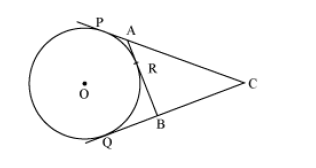
\includegraphics[width=0.5\columnwidth,center]{./fig/1.png}
	\caption{}
	\label{fig1}
 \end{figure} 
\item In Fig \ref{fig2}, $DE \parallel BC$ in ABC such that BC = 8cm, AB = 6cm and DA = 1.5cm. Find DE.
\begin{figure}[h!]
    \centering
    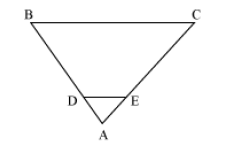
\includegraphics[width=0.5\columnwidth,center]{./fig/2.png}
	\caption{}
	\label{fig2}
 \end{figure} 
\item  If $5x=\sec\theta$ and $\myvec{\frac{5}{x}=\tan\theta}$ find the value of $5(x^2-\frac{1}{x^2})$ \\
\item What is the distance between the points A (c,0) and B(0,–c)? \\
\item  In a $\triangle ABC $, right-angled at C, AC = 6cm and AB = 12cm. Find $\angle$ A. \\
\item  The slant height of the frustum of a cone is 5cm. If the difference between the radii of its two circular ends is 4 cm, write the height of the frustum. \\
\item  A die is thrown once. What is the probability of getting a number greater than 4?
\end{enumerate}
\section{Section B}
\renewcommand{\theequation}{\theenumi}
\begin{enumerate}[label=\thesection.\arabic*.,ref=\thesection.\theenumi]
\numberwithin{equation}{enumi}
\item  For what value of k, is 3 a zero of the polynomial $2x2+x+k$? \\
\item  Find the value of m for which the pair of linear equations $2x+3y–7=0$ and $(m–1)x+(m+1)y =(3m–1)$ has infinitely many solutions. \\
\item  Find the common difference of an A.P. whose first term is 4, the last term is 49 and the sum of all its terms is 265. \\
\item In Fig \ref{fig3}, there are two concentric circles with centre O and of radii 5 cm and 3 cm. From an external point P, Tangents PA and PB are drawn to these circles. If AP = 12 cm, find the length of BP. \pagebreak
\begin{figure}[h!]
    \centering
    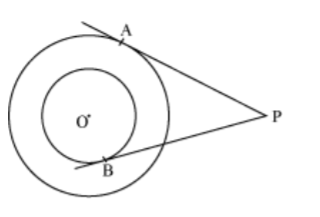
\includegraphics[width=0.5\columnwidth,center]{./fig/3.png}
	\caption{}
	\label{fig3}
 \end{figure}
\item  Without using trigonometric tables, evaluate the following:
\begin{align}
\frac{cos 70\degree}{3 sin 20\degree}+\frac{4(sec^2 59\degree- cot^231\degree}{3}-\frac{2}{3}sin 90\degree \nonumber
\end{align} \\
\end{enumerate}
\section{Section C}
\renewcommand{\theequation}{\theenumi}
\begin{enumerate}[label=\thesection.\arabic*.,ref=\thesection.\theenumi]
\numberwithin{equation}{enumi}
\item Prove that $\sqrt3$ is an irrational number \\
\item \begin{enumerate}
\item Solve the following pair of linear equations for x and y: $\frac{b}{a}x+\frac{a}{b}y=a^2+b^2$ and $x+y=2ab$ \\
\item The sum of the numerator and the denominator of a fraction is 4 more than twice the numerator. If 3 is added to each of the numerator and denominator, their ratio becomes 2:3. Find the fraction. \\
\end{enumerate}
\item In an A.P., the sum of its first ten terms is – 80 and the sum of its next ten terms is -280. Find the A.P. \\
\item  In Fig \ref{fig4}, ABC is an isosceles triangle in which AB = AC. E is a point on the side CB produced, such that \\ $FE \perp AC$. If $AD \perp CB$, prove that: \\ AB$\times$ EF = AD $\times$ EC
\begin{figure}[h!]
    \centering
    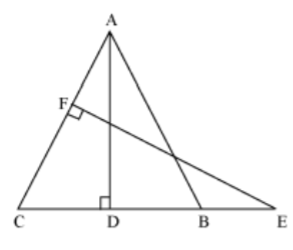
\includegraphics[width=0.5\columnwidth,center]{./fig/4.png}
	\caption{}
	\label{fig4}
 \end{figure}
\item \begin{enumerate}
\item Prove the following:
\begin{align}
(1+\cot A - \cosec A)(1 + \tan A + \sec A) \nonumber \\=2 \nonumber
\end{align}
\item Prove the following:
\begin{align}
\sin A(1+\tan A)+\cos A (1+\cot A)  \nonumber \\ = \sec A + \cosec A \nonumber
\end{align}
\end{enumerate}
\item Construct a triangle ABC in which AB = 8 cm, BC = 10 cm and AC = 6 cm. Then construct another triangle whose sides are $\frac{4}{5}$ of the corresponding sides of $\triangle ABC$. \\
\item Point P divides the line segment joining the points A (–1, 3) and B (9, 8) such  that
\begin{align}
\frac{AP}{BP}=\frac{k}{1} \nonumber
\end{align}
If P lies on the line $x–y+2=0$, find the value of k. \\
\item If the points (p, q); (m, n) and (p – m, q – n) are collinear, show that pn = qm. \\
\item \begin{enumerate}
\item The rain-water collected on the roof of a building, of dimensions $22 m \times 20 m$, is drained into a cylindrical vessel having base diameter 2 m and height 3.5 m. If the vessel is full up to the brim, find the height of rain-water on the roof [Use $\pi = \frac{22}{7}$] \\
\item In Fig \ref{fig5}, AB and CD are two perpendicular diameters of a circle with centre O. If OA = 7 cm, find the area of the shaded region. [Use $\pi=\frac{22}{7}$]
\begin{figure}[h!]
    \centering
    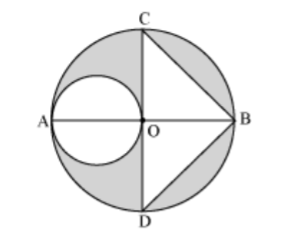
\includegraphics[width=0.5\columnwidth,center]{./fig/5.png}
	\caption{}
	\label{fig5}
 \end{figure}
\end{enumerate}
\item A bag contains cards which are numbered from 2 to 90. A card is drawn at random from the bag. Find the probability that it bears \\
\begin{enumerate}
\item a two digit number,
\item a number which is a perfect square. 
\end{enumerate}
\end{enumerate}
\section{Section D}
\renewcommand{\theequation}{\theenumi}
\begin{enumerate}[label=\thesection.\arabic*.,ref=\thesection.\theenumi]
\numberwithin{equation}{enumi}
\item A girl is twice as old as her sister. Four years hence, the product of their ages (in years) will be 160. Find their present ages. \\
\item In a triangle, if the square of one side is equal to the sum of the squares of the other two sides, then prove that the angle opposite the first side is a right angle. \\
Using the above, do the following: \\ In an isosceles triangle PQR, PQ = QR and $PR^2=2PQ^2$. Prove that $\angle Q$ is a right angle. \\
\item \begin{enumerate}
\item A man on the deck of a ship, 12 m above water level, observes that the angle of elevation of the top of a cliff is $60\degree$ and the angle of depression of the base of the cliff is $30\degree$. Find the distance of the cliff from the ship and the height of the cliff. [Use $\sqrt{3}= 1.732$] \\
\item The angle of elevation of a cloud from a point 60 m above a lake is $30\degree$ and the angle of depression of the reflection of the cloud in the lake is $60\degree$. Find the height of the cloud from the surface of the lake. \\
\end{enumerate}
\item The surface area of a solid metallic sphere is 616 $cm^2$. It is melted and recast into a cone of height 28 cm. Find the diameter of the base of the cone so formed.  [Use $\pi=\frac{22}{7}$] \\
\end{enumerate}
\end{document}